\documentclass[10pt]{beamer}

\usepackage[brazil]{babel}
\usetheme[progressbar=frametitle]{metropolis}
\usepackage{appendixnumberbeamer}
\usepackage[numbers,sort&compress]{natbib}
\bibliographystyle{plainnat}
\usepackage{caption}

\usepackage{algorithm, algpseudocode}  % Pacote para escrever algoritmos em pseudo-codigo

\usepackage{MnSymbol}
\newtheorem{teo}{\scshape Teorema}


\usepackage{booktabs}
\usepackage[scale=2]{ccicons}

\usepackage{xspace}
\newcommand{\themename}{\textbf{\textsc{metropolis}}\xspace}

\title{Geradores de homologia persistente e aplicações}
\date{13 de Novembro de 2019}
\author{Carlos Ronchi \\
        Marcio Gameiro}
\institute{Universidade de São Paulo}
\titlegraphic{\hfill
\includegraphics[height=1.0cm]{images/icmc_logo.png}}

\newcommand{\source}[1]{\caption*{Fonte: {#1}} }

\begin{document}

\maketitle

\begin{frame}
    \tableofcontents 
\end{frame}

\section{Introdução à homologia persistente}

\begin{frame}{Primeiros Passos}
    \begin{figure}
        \centering
        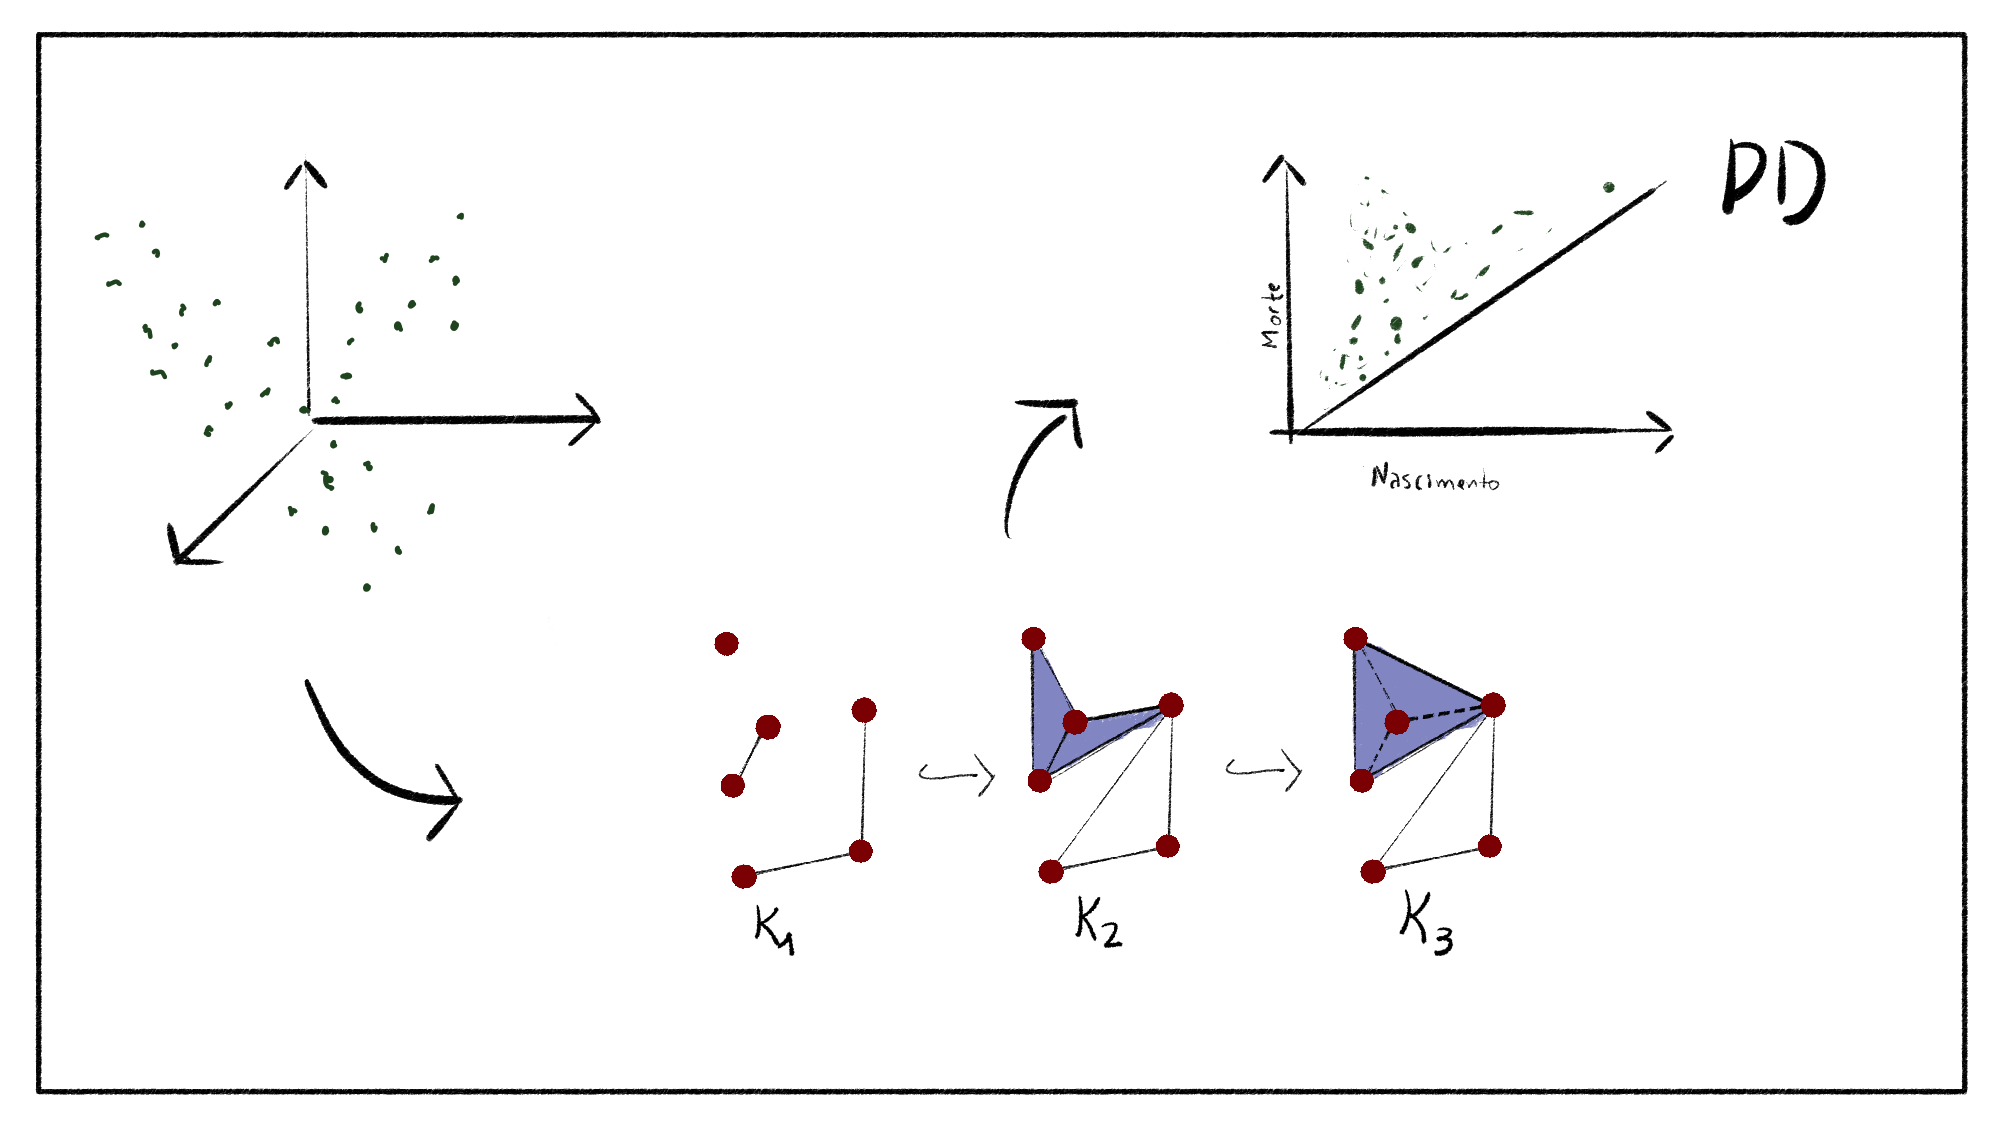
\includegraphics[width=0.9\textwidth]{images/StepsHomPers.png}
    \end{figure}
\end{frame}

\begin{frame}{Tipos de complexos}
    \begin{figure}
        \centering
        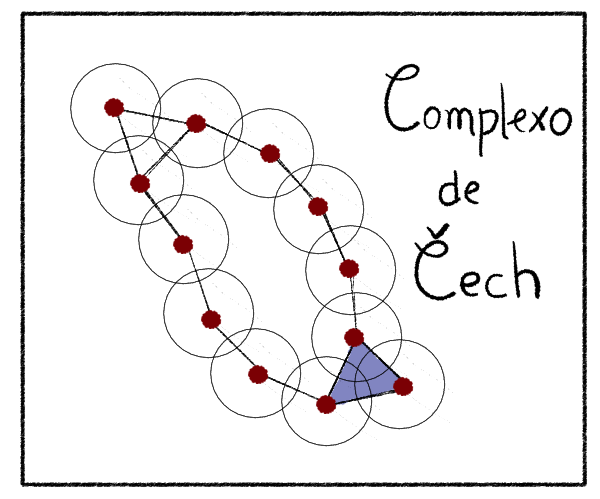
\includegraphics[width=0.8\textwidth]{../images/ComplexCech.png}
    \end{figure}   
\end{frame}

\begin{frame}{Tipos de complexos}
    \begin{figure}
        \centering
        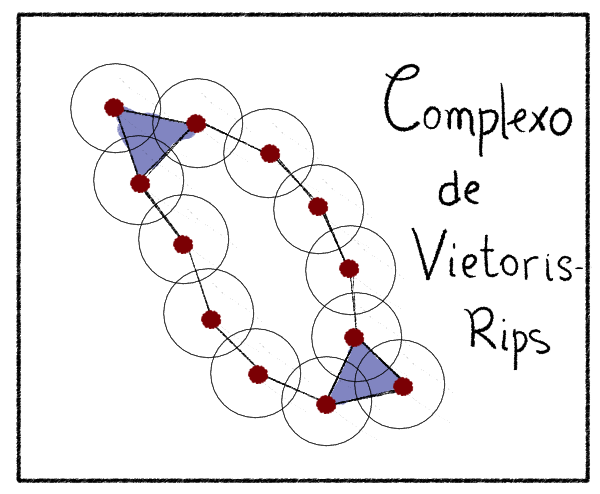
\includegraphics[width=0.8\textwidth]{../images/ComplexRips.png}
    \end{figure}   
\end{frame}

\begin{frame}{Tipos de complexos}
    \begin{figure}
        \centering
        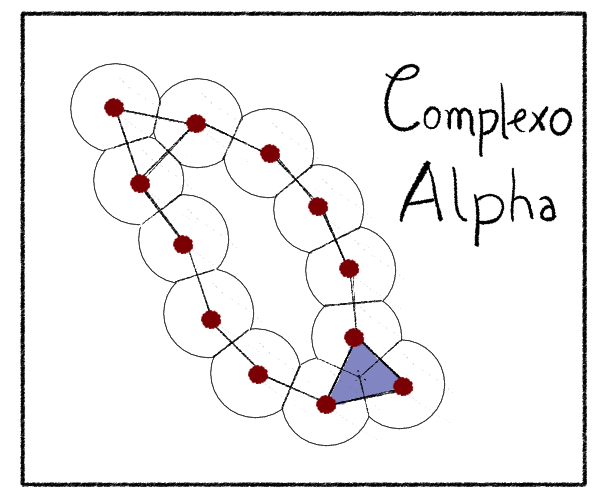
\includegraphics[width=0.8\textwidth]{../images/ComplexAlpha.png}
    \end{figure}   
\end{frame}

\begin{frame}{Propriedades dos complexos}
    Seja $r > 0$ fixado, então
    \begin{itemize}
        \item $C^r(X) \subset V^r(X) \subset C^{2r}(X)$
        \item $A^r(X) \subset C^r(X)$
    \end{itemize} 
\end{frame}

\begin{frame}{Filtração}
    Para um complexo simplicial $K$ fixado, definimos sua filtração como 
    \begin{equation*}
        K_1 \subset K_2 \subset \dots \subset K_n = K,
    \end{equation*}
    em que $K_i$ é um complexo simplicial, para todo $i \in \{1, \dots, n\}$. 
\end{frame}

\begin{frame}{Homologia Persistente}
    \centering
    {\Large Filtração $\rightarrow$ $(H_m(K_1) \to H_m(K_2) \to \dots \to H_m(K_n))$}
\end{frame}

\begin{frame}{Diagrama de persistência} 
     \begin{figure}
        \centering
        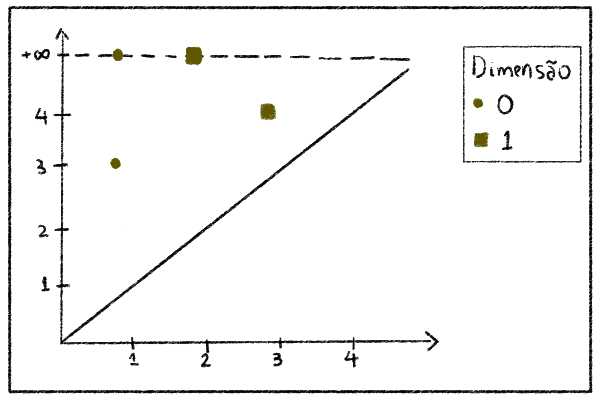
\includegraphics[width=0.8\textwidth]{../images/persdiag_ex.png}
    \end{figure}   
\end{frame}

\begin{frame}{Exemplo}
    \begin{figure}
        \centering
        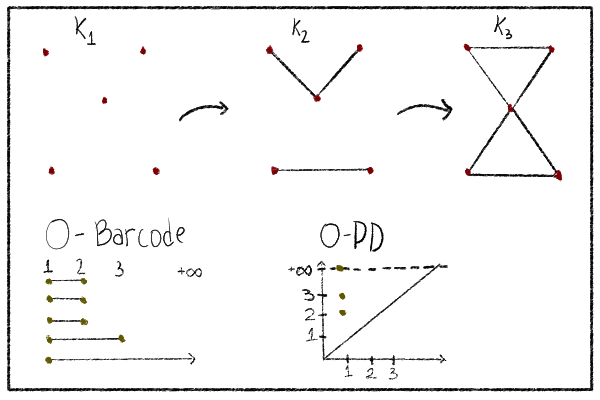
\includegraphics[width=0.8\textwidth]{../images/filt_bar_pd.png}
    \end{figure}
\end{frame}

\section{Módulos de persistência}

\begin{frame}{Formalização}
    \centering
    {\Large Como podemos formalizar esse processo e garantir a existência
    do diagrama de persistência?}
\end{frame} 

\begin{frame}{Definição}
    \begin{itemize}
        \item Seja $T = \mathbb{R}$ um poset e $(V_t)_{t \in T}$ uma sequência de espaços vetoriais
        \item Sejam $v_t^s \colon V_s \to V_t$, $s,t \in T$ tais que 
                \begin{equation*}
                    v^t_r \circ v^s_t = v^s_r.
                \end{equation*}
    \end{itemize}
\end{frame}

\begin{frame}{Módulos Intervalares}
    Seja $J \subset T$ um intervalo, o módulo intervalar $\mathfrak{I} = \mathbf{k}^J$ 
    é o $\mathbf{T}$-módulo de persistência com os espaços vetoriais 
    \begin{equation*}
    I_t = \left\{
    \begin{split}
        & \mathbf{k} \text{ se } t \in J \\
        & 0 \text{ caso contrário,}
    \end{split}
    \right.
\end{equation*} 
e as aplicações lineares
\begin{equation*}
    i_t^s = \left\{
    \begin{split}
        & id \text{ se } s,t \in J \\
        & 0 \text{ caso contrário.}
    \end{split}
    \right.
\end{equation*}

\end{frame}

\begin{frame}{Diagrama de persistência}
    \centering
    {\Large Sob quais condições temos que o módulo de persistência é decomponível?} 
\end{frame}

\begin{frame}{Resposta}
    \begin{teo}{(Gabriel, Auslander, Ringel-Tachikawa, Webb, Crawley-Boevey)}\label{teo:crawley}
    Seja $\mathfrak{V}$ um módulo de persistência sobre $\mathbf{T} \subset \mathbb{R}$. Então $\mathfrak{V}$
    pode ser decomposto como um soma direta de módulos intervalares sob as seguintes condições:
    \begin{itemize} 
        \item $\mathbf{T}$ é um conjunto finito;
        \item cada $V_t$ é um espaço vetorial de dimensão finita. 
    \end{itemize}
    Por outro lado, existe um módulo de persistência sob $\mathbb{Z}$ que não admite uma decomposição intervalar. 
\end{teo}  
\end{frame}

\section{Geradores ótimos} 

\begin{frame}{Quando os ciclos são ótimos?}
    \begin{figure}
        \centering
        
\includegraphics[width=0.6\textwidth]{images/ciclotimo}
    \end{figure}
\end{frame}

\begin{frame}{Obtenção dos ciclos ótimos}
    \begin{figure}
        \centering
        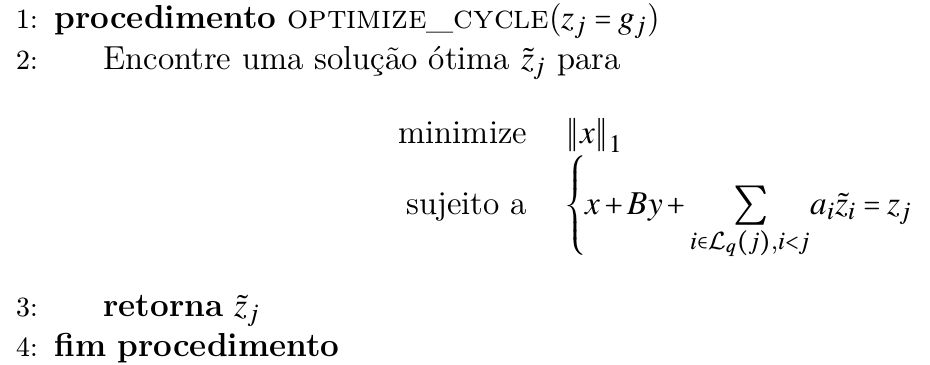
\includegraphics[width=0.8\textwidth]{images/gerotimo.png}
    \end{figure}
\end{frame}

\begin{frame}{Geradores}
    \begin{figure}
        \centering
        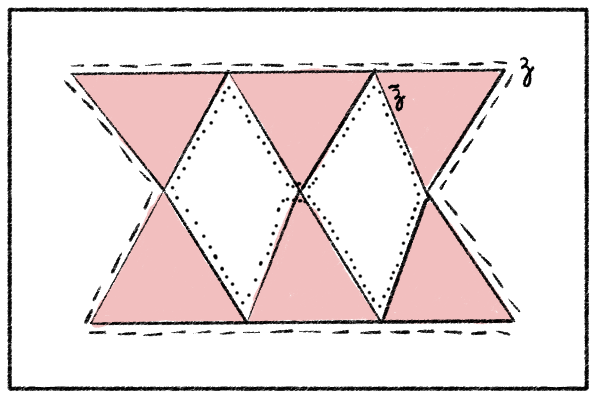
\includegraphics[width=0.8\textwidth]{../images/nonoptcyc.png}
    \end{figure}
\end{frame}

\section{Desenvolvimento computacional de proteínas}

\begin{frame}{Aminoácidos}
    \begin{figure}
        \centering
        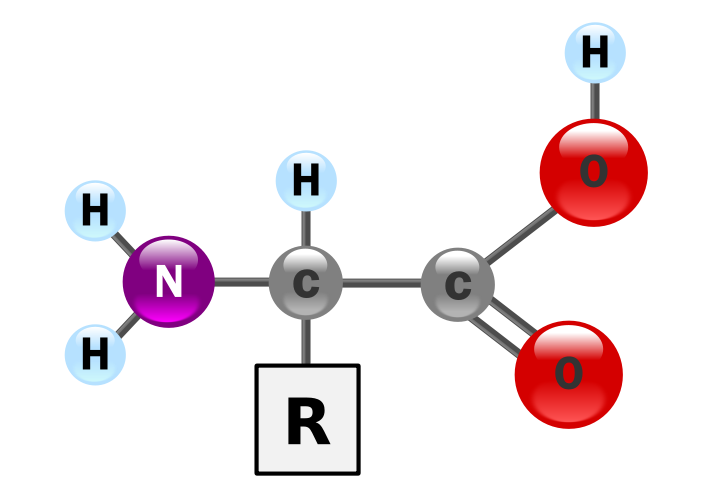
\includegraphics[width=0.8\textwidth]{images/aminoacid.png}
        \caption*{Fonte: Wikimedia Commons}
    \end{figure}  
\end{frame}

\begin{frame}{Enovelamento}
    \begin{figure}
        \centering
        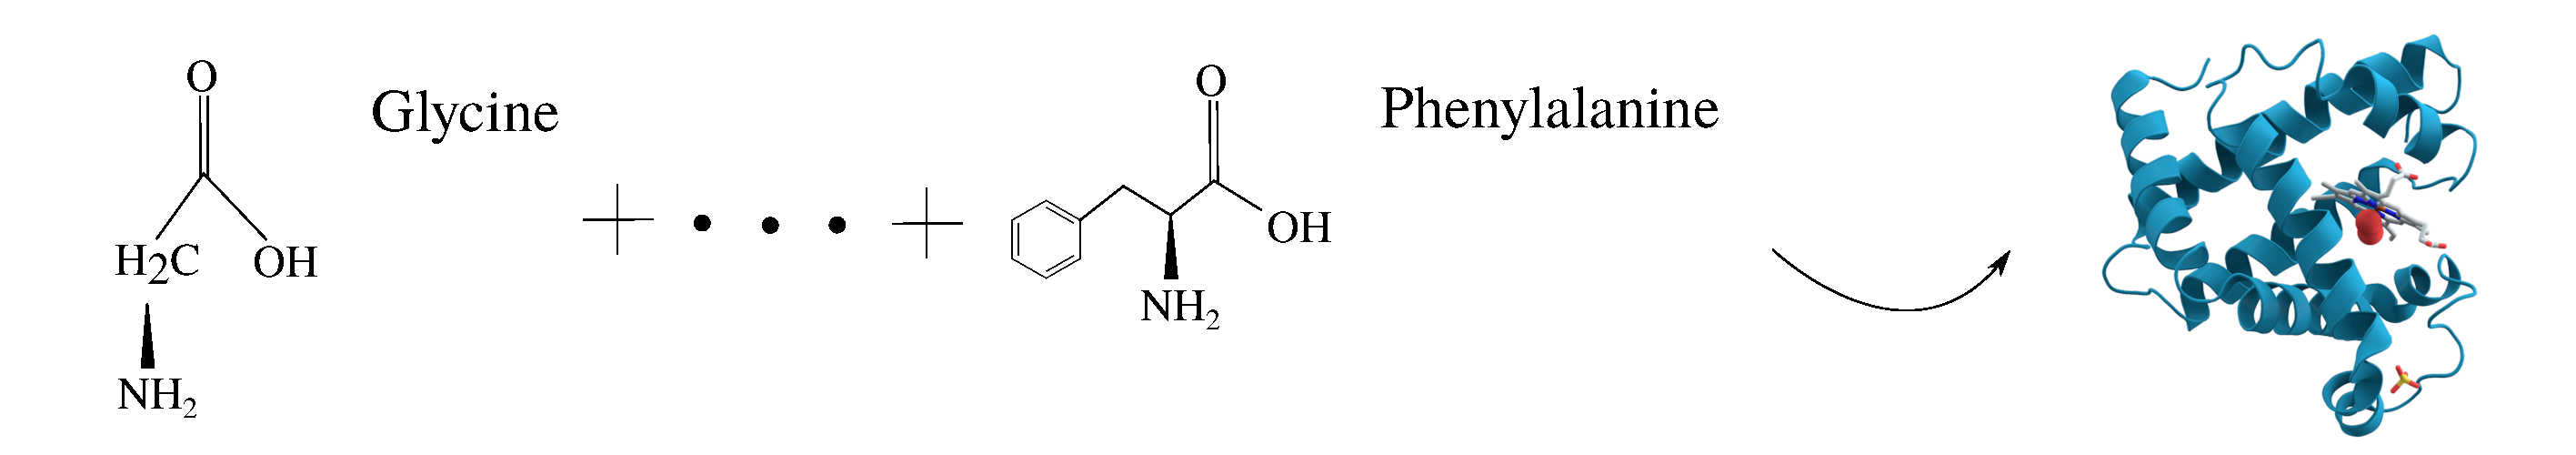
\includegraphics[width=1.0\textwidth]{images/aminoplusprotein.pdf}
    \end{figure} 
\end{frame}

\begin{frame}{Proteínas simuladas}
    \begin{figure}
        \centering
        
\includegraphics[width=1.0\textwidth]{images/computationalprotein.pdf}
    \end{figure} 
\end{frame}

\section{Experimentos - Rocklin}

\begin{frame}{Estabilidade da proteína} 
   \begin{figure}
        \centering
        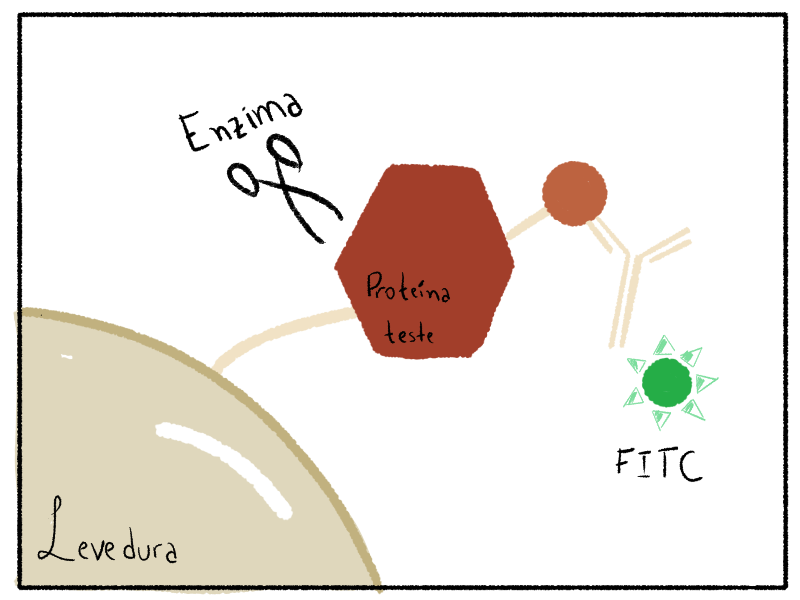
\includegraphics[width=0.8\textwidth]{../images/yeast_cell.png}
    \end{figure} 
\end{frame}

\begin{frame}{Prevendo a estabilidade}
  \begin{table}
      \begin{tabular}{@{}ccc@{}}
      \toprule
      Modelo          & RMSE & Erro percentual (\%) \\ \midrule
      Random Forest & 0,419         & 11,381          \\ \bottomrule
      \end{tabular}
      \label{tab:rocklin}
  \end{table}
\end{frame}

\begin{frame}{Metodologia}
    \begin{figure}
        \centering
        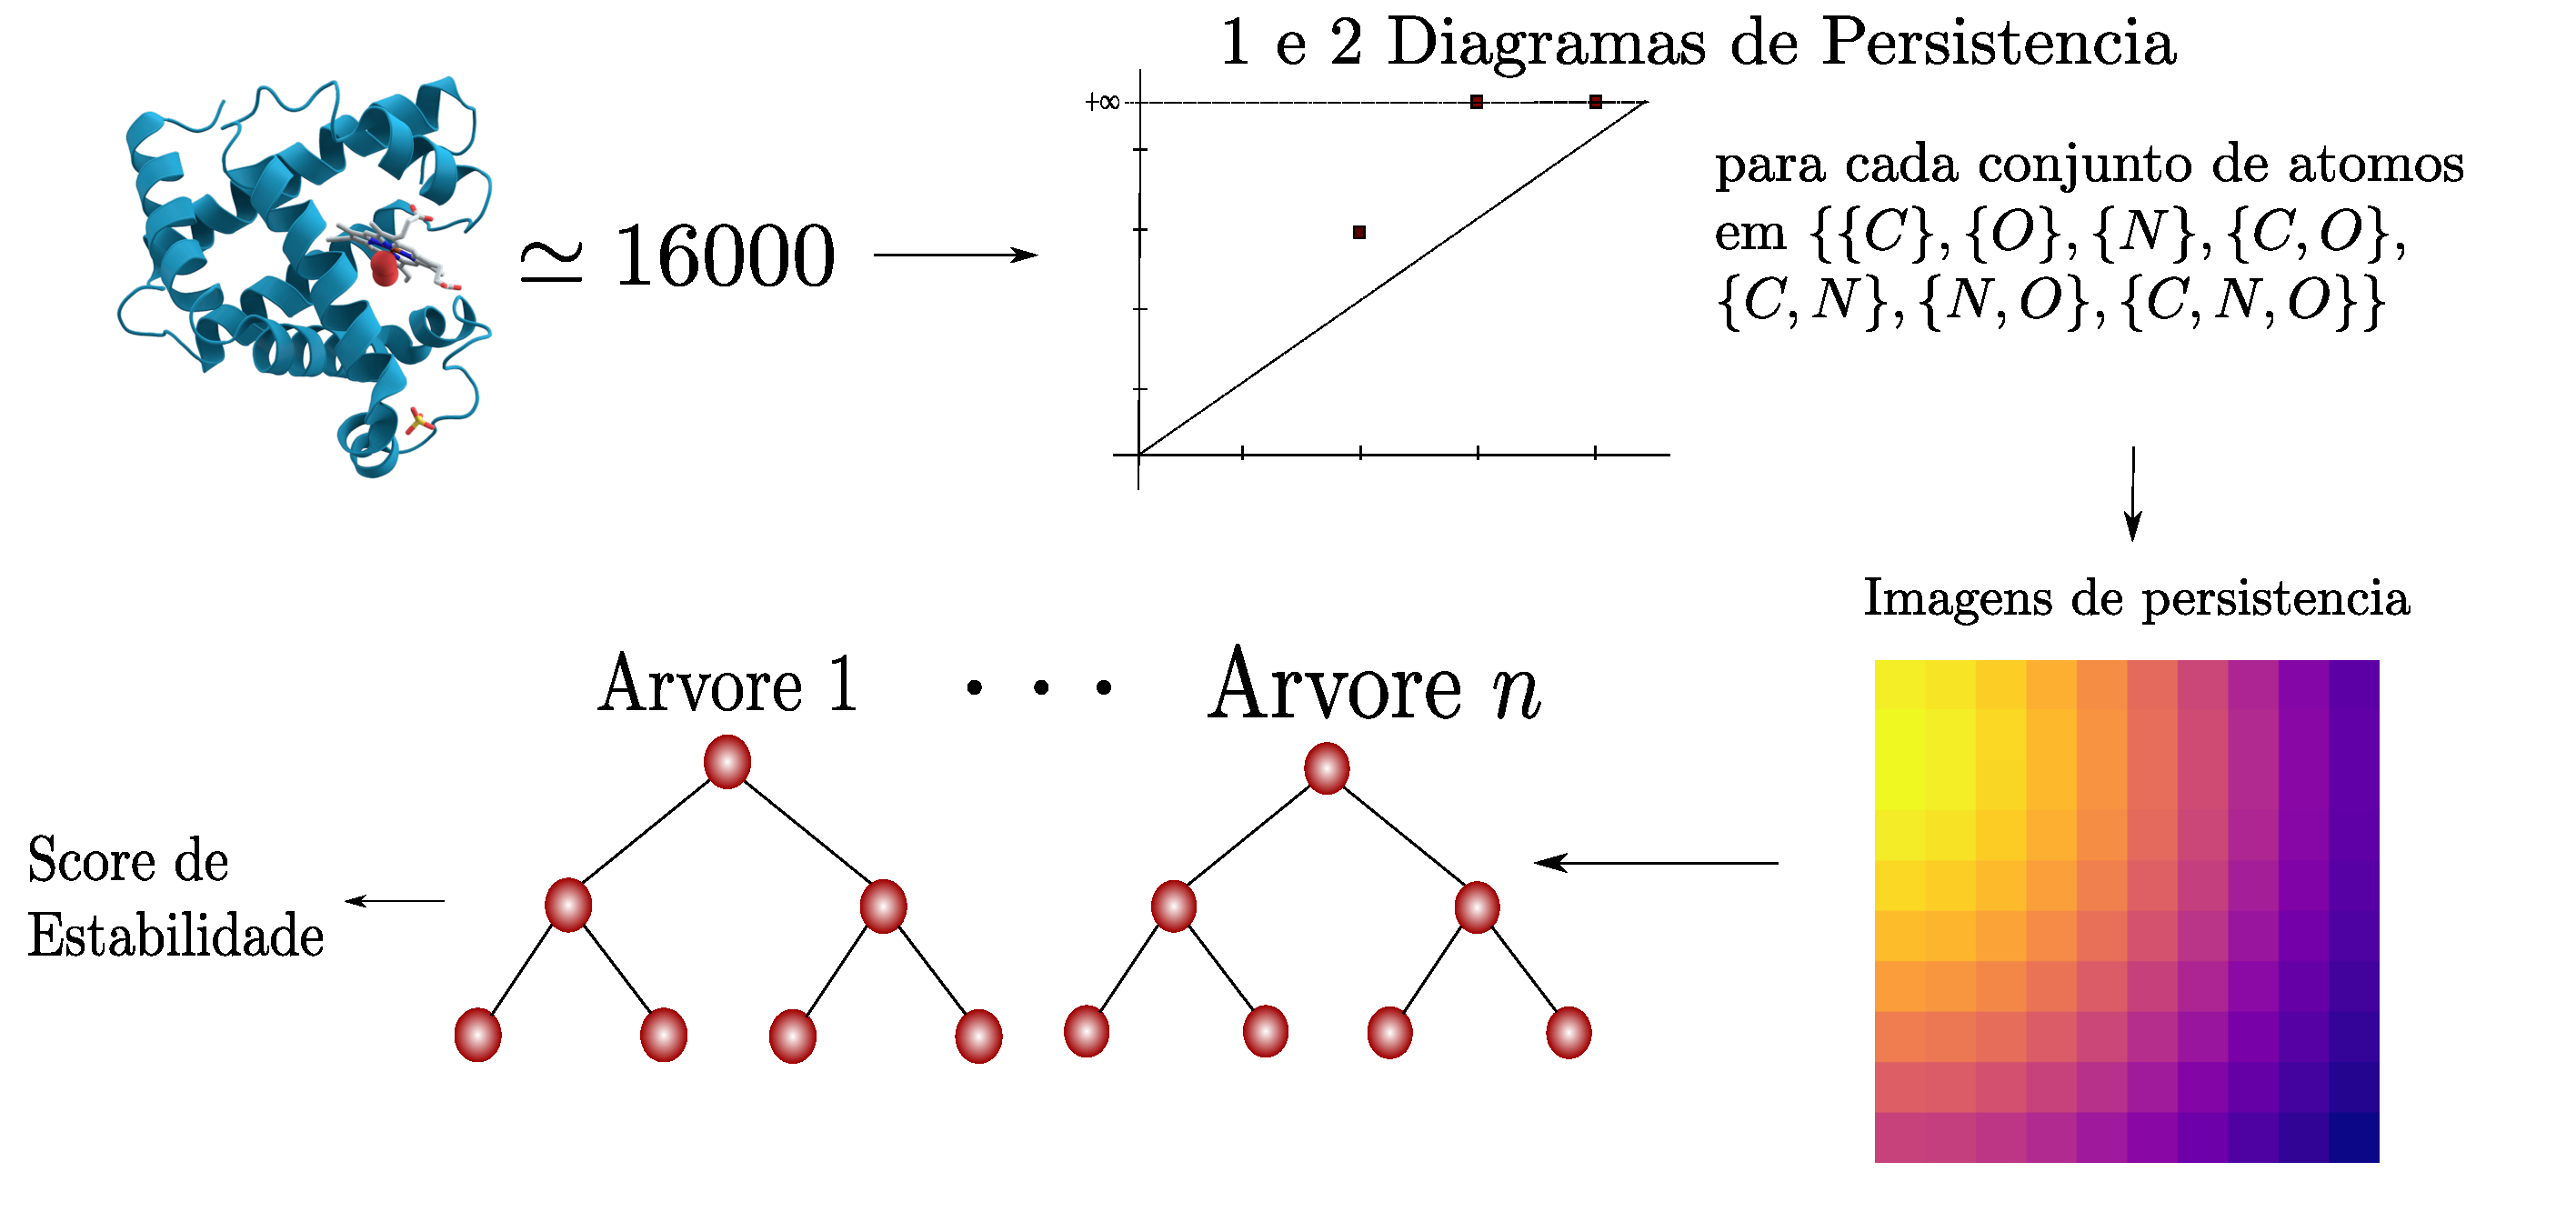
\includegraphics[width=0.99\textwidth]{../images/proteinpipeline.pdf}
    \end{figure}
\end{frame}

\begin{frame}{Resultados}
    \begin{table}[]
    \begin{tabular}{@{}cccc@{}}
    \toprule
    Modelo              & RMSE   & Erro Percentual (\%) \\ \midrule
    Regressão linear & 0,5046 & 13,69              \\
    Random Forest I        & 0,4877 & 13,24              \\
    Random Forest II    & 0,4874 & 13,23              \\
    GBoost ótimo     & 0,4770 & 12,95              \\
    Modelo Rocklin \footnote{Science  14 Jul 2017:\\
Vol. 357, Issue 6347, pp. 168-175\\
DOI: 10.1126/science.aan0693} & 0,419 & 11,381 \\ 
    \bottomrule
    \end{tabular}
    \caption{Variância: $0,7$, Grid: 5x4.}
  \end{table}
\end{frame}

\begin{frame}{Análise}
  \begin{figure}
    \centering
    \begin{minipage}{0.45\textwidth}
        \centering
        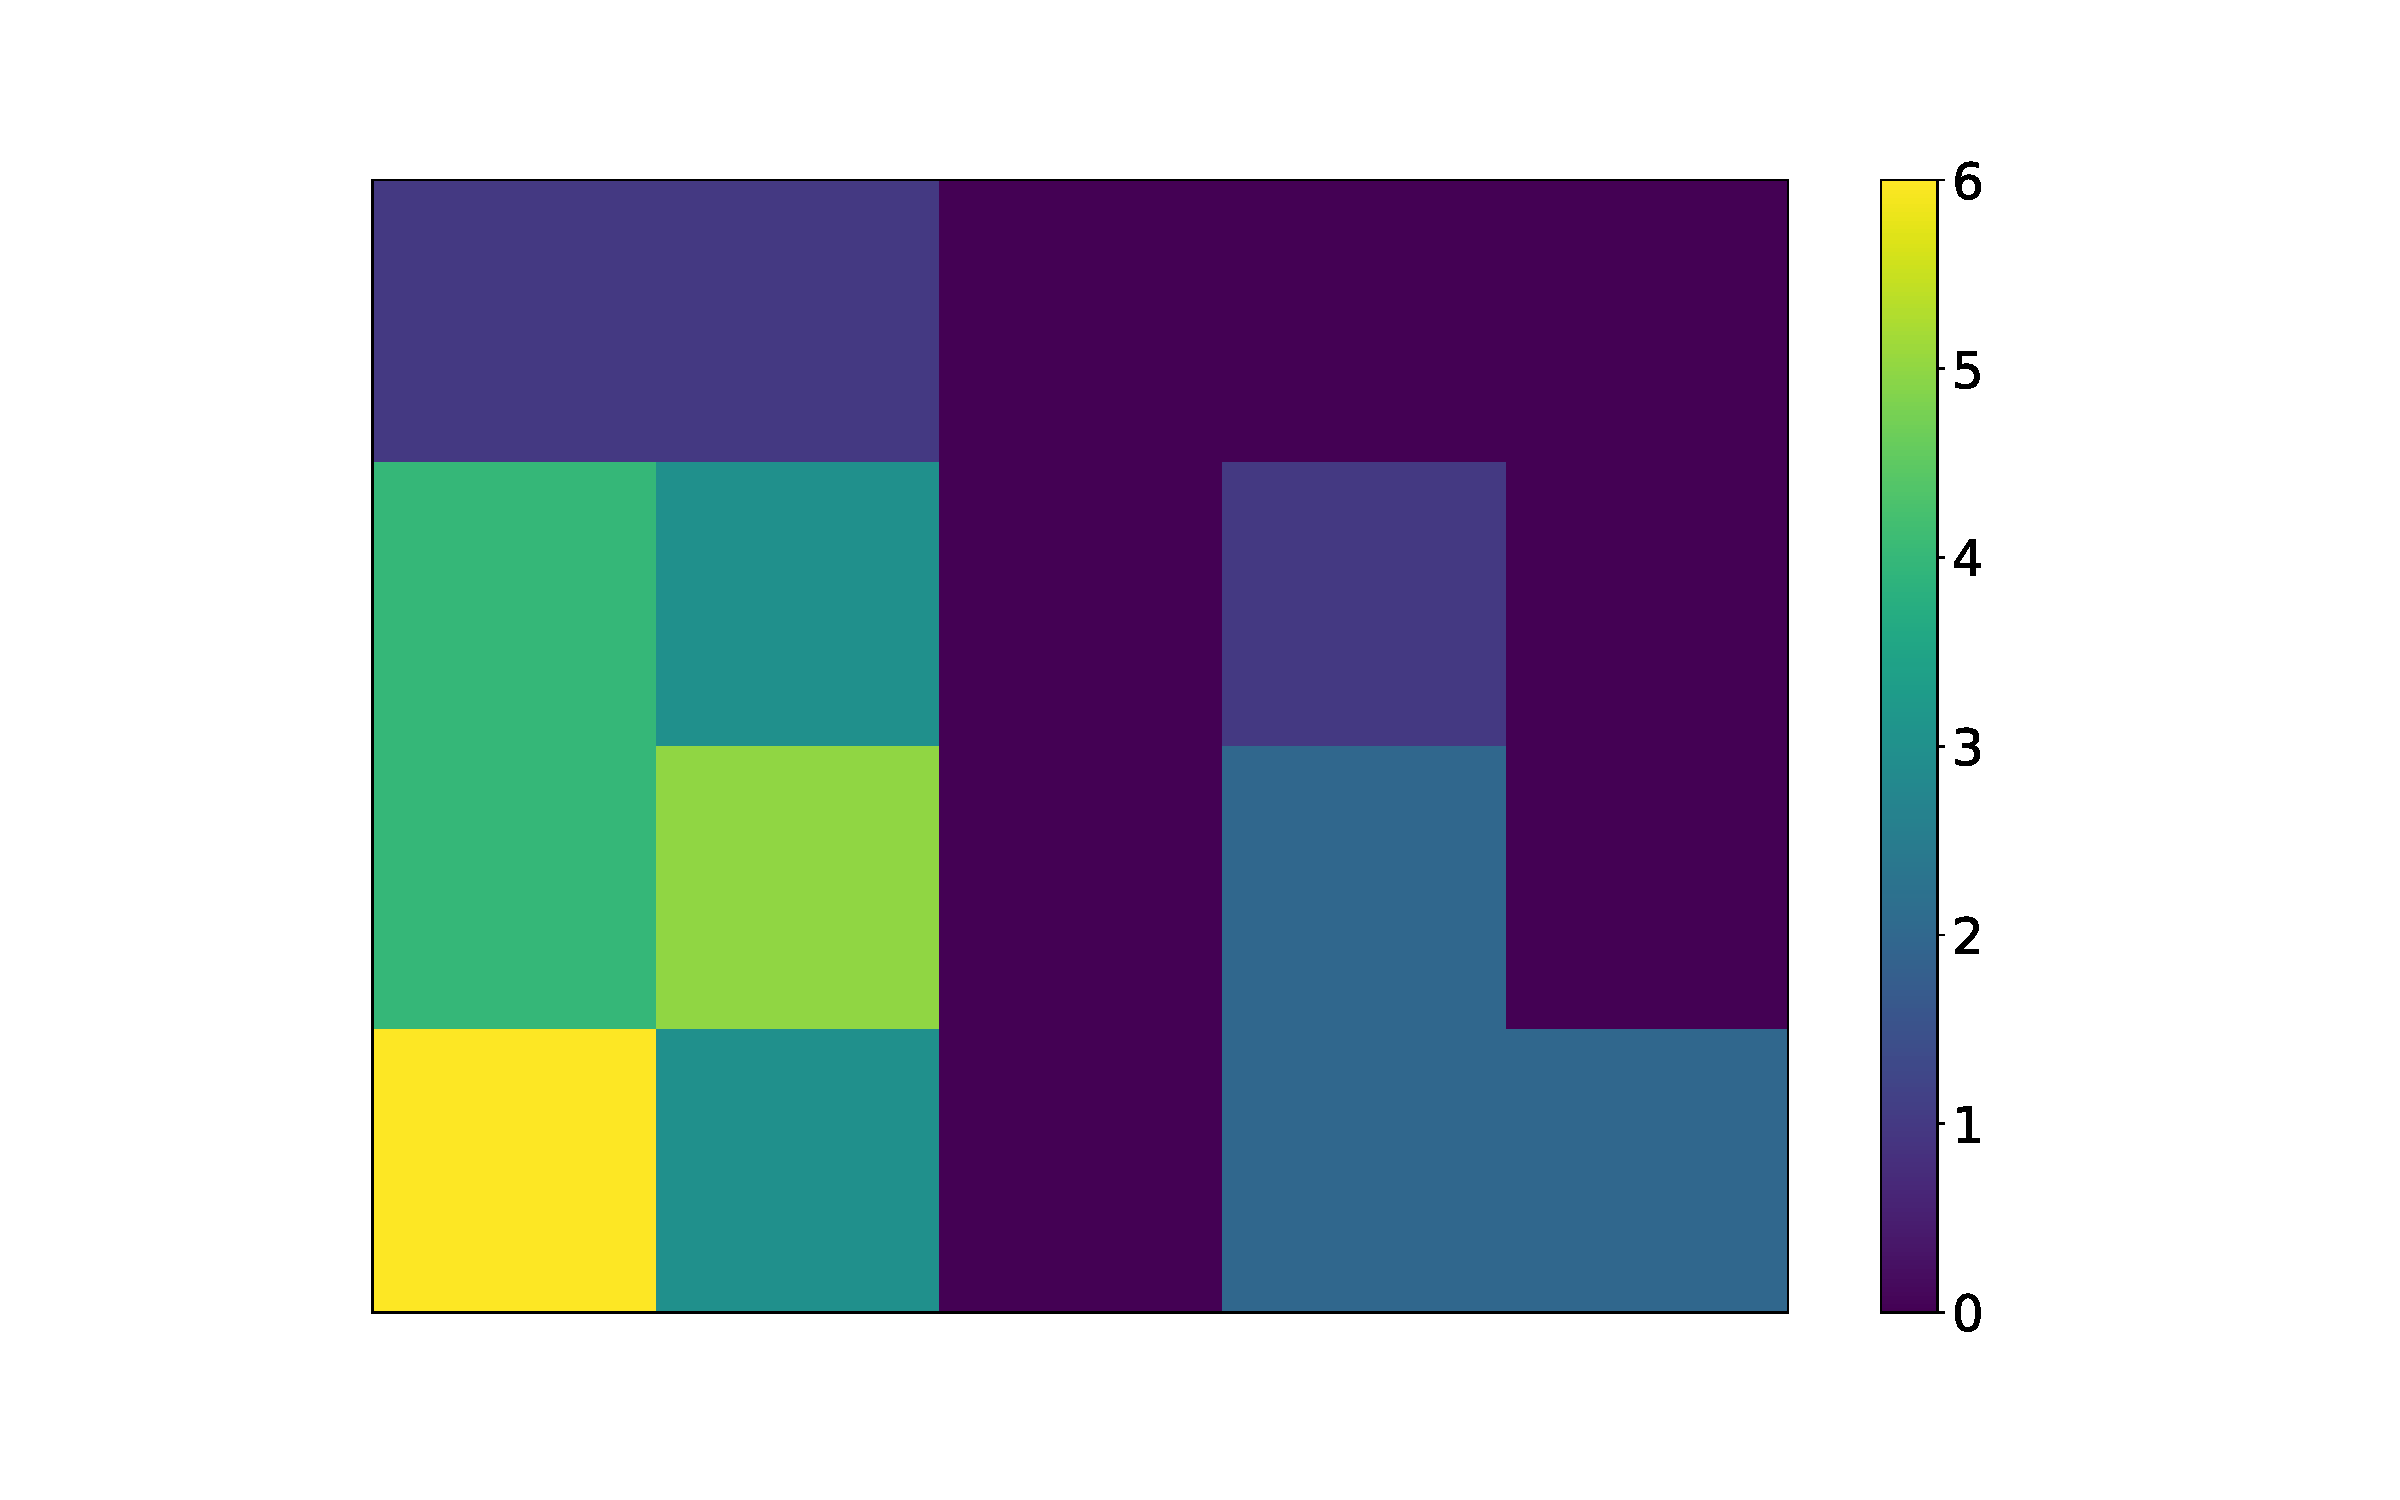
\includegraphics[width=1.1\textwidth]{images/heatmap_1.pdf} % first figure itself
        \caption{Dimensão 1}
    \end{minipage}\hfill
    \begin{minipage}{0.45\textwidth}
        \centering
        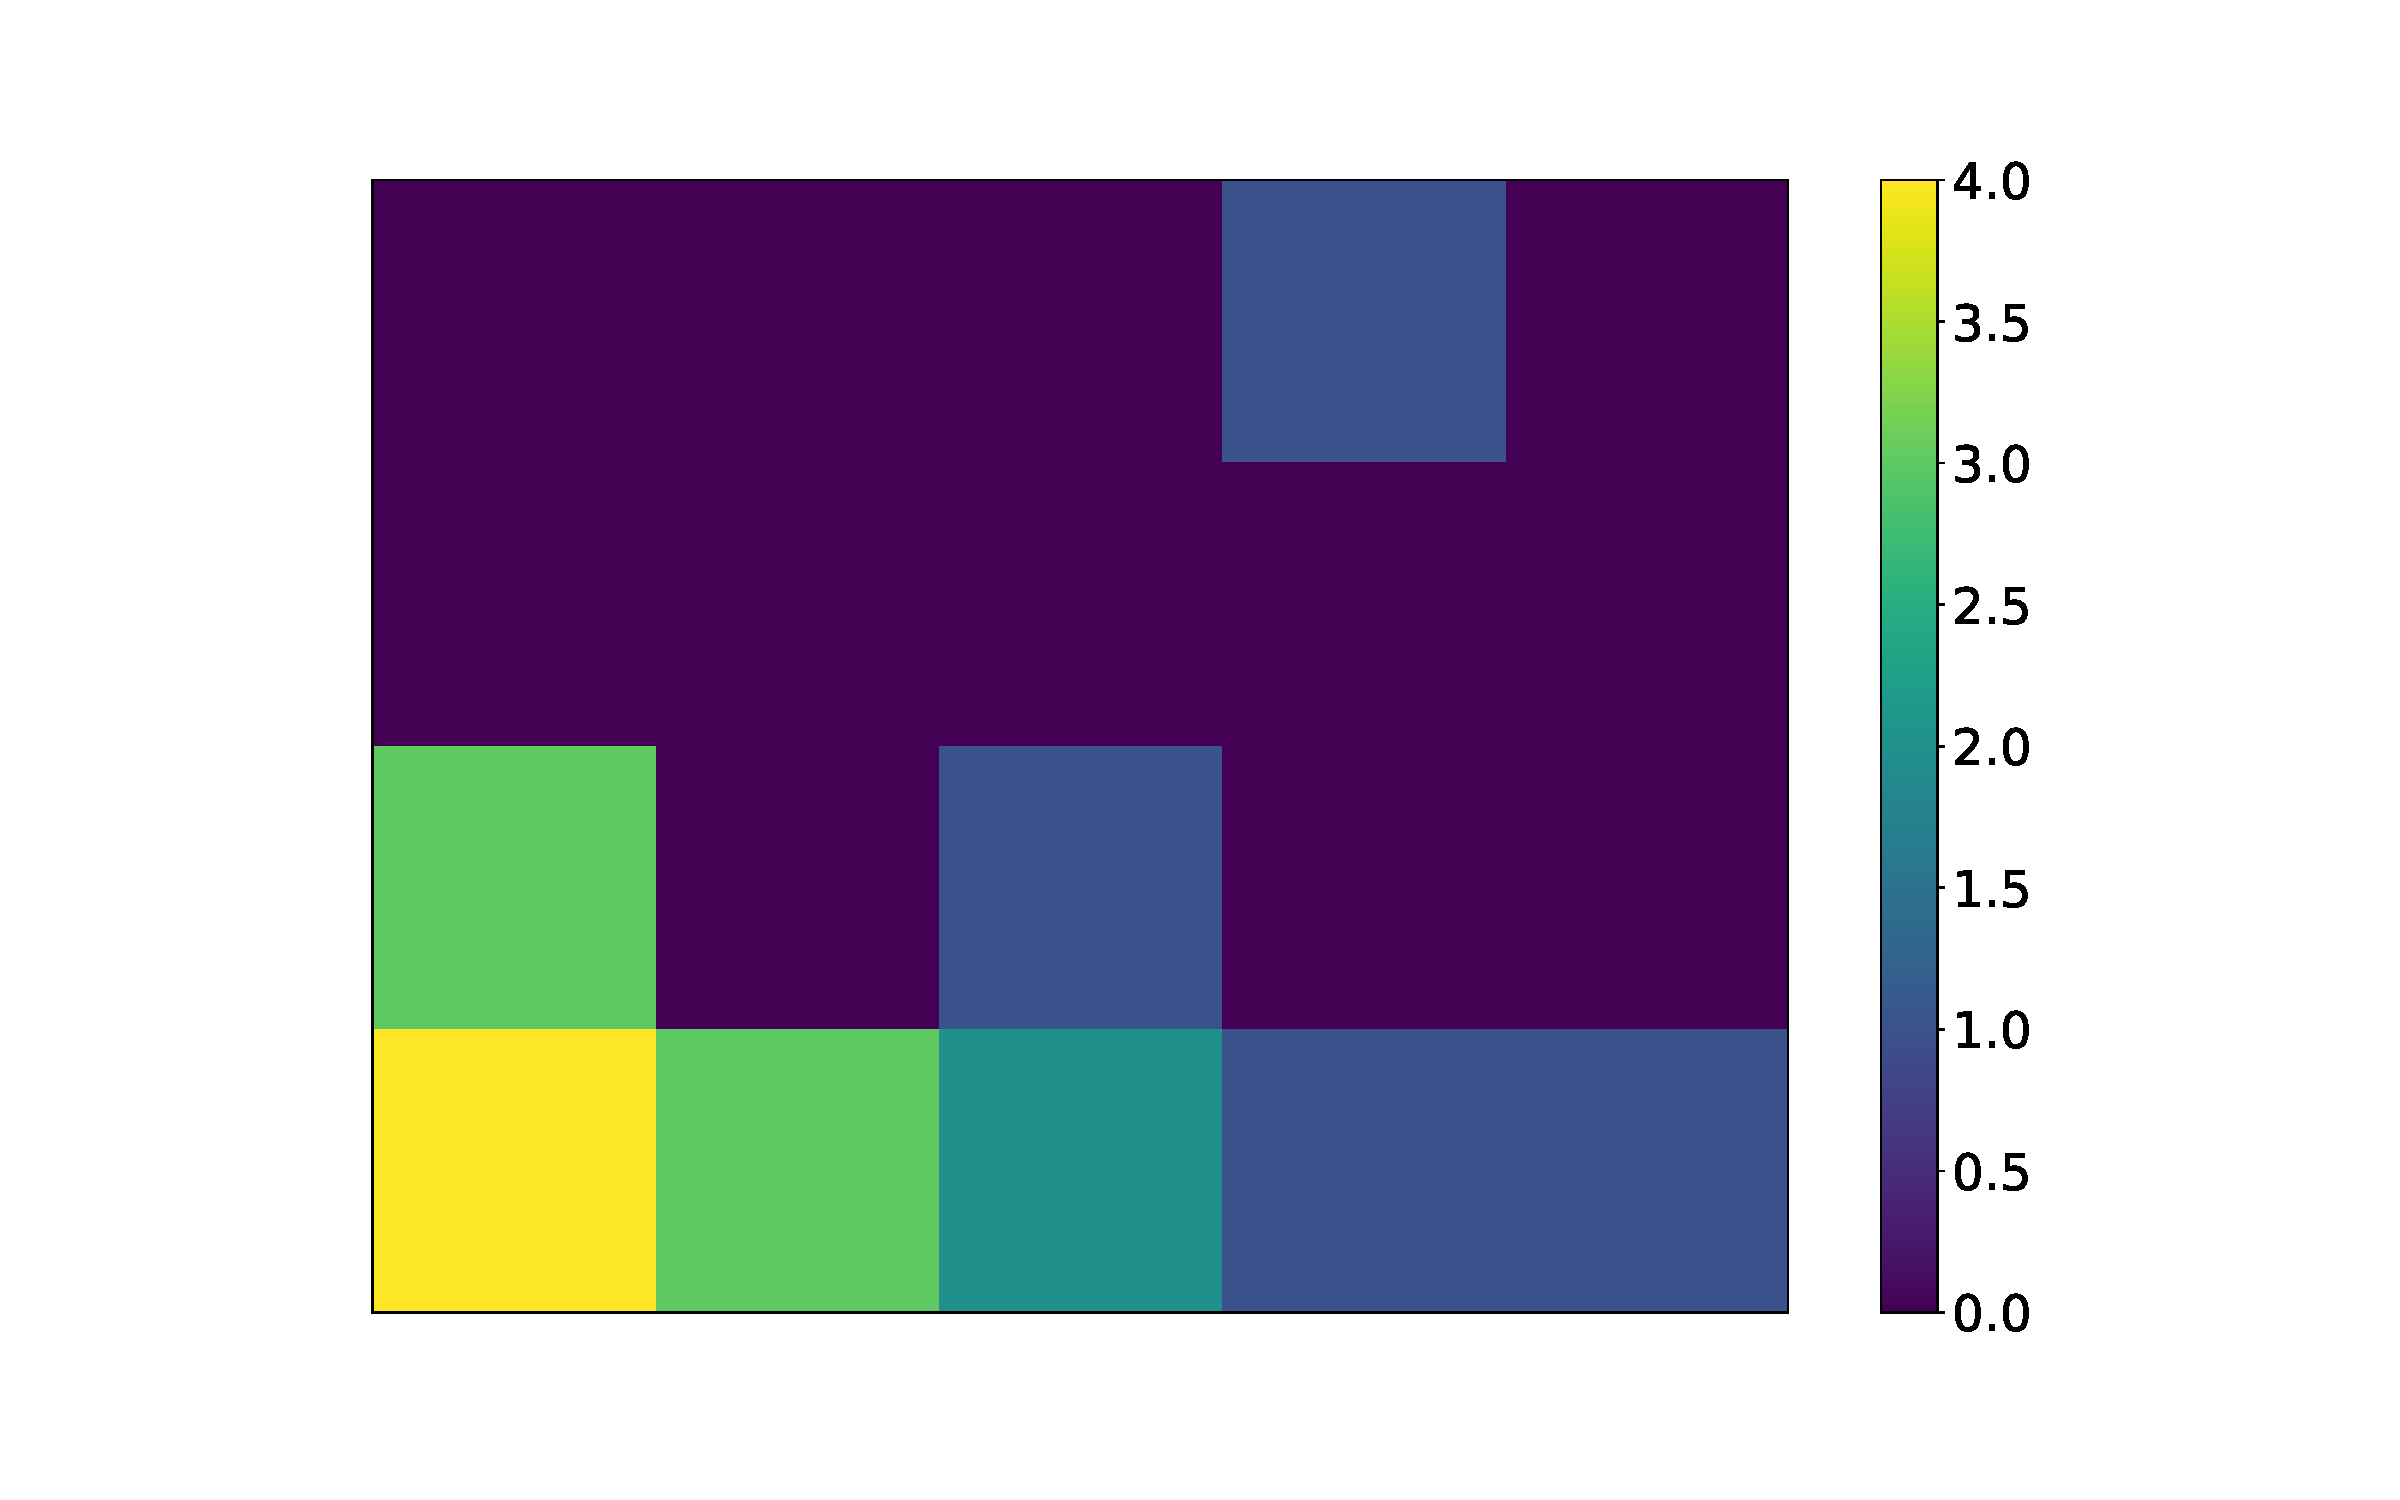
\includegraphics[width=1.1\textwidth]{images/heatmap_2} % second figure itself
        \caption{Dimensão 2}
    \end{minipage}
  \end{figure}
\end{frame}

\begin{frame}{Ciclos e átomos}
    \begin{figure}
        \centering
        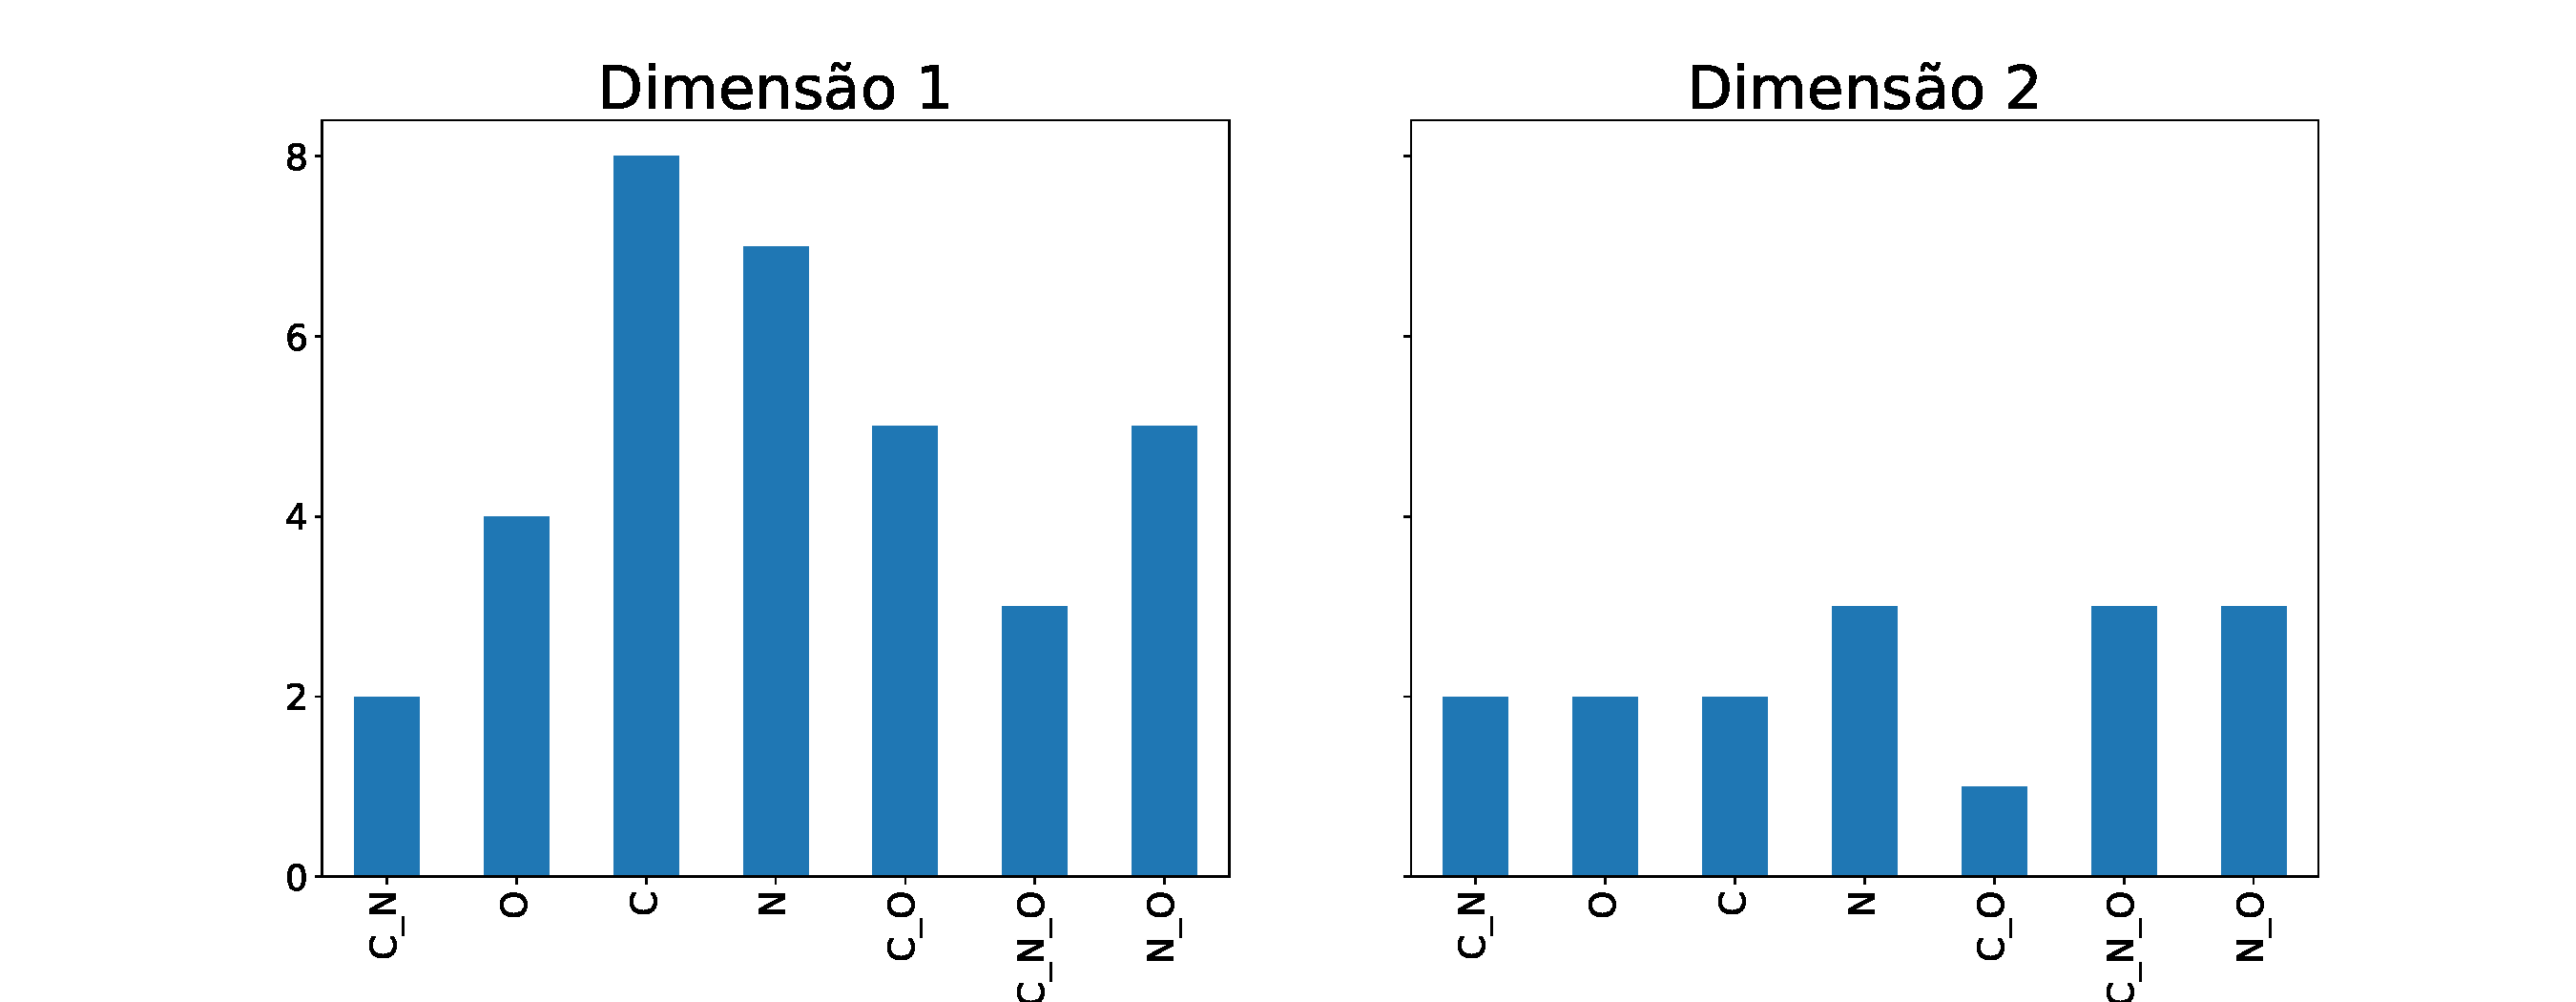
\includegraphics[width=1.0\textwidth]{images/plt_dim.pdf}
    \end{figure}
\end{frame}

\section{Experimentos - Sagar}

\begin{frame}{Propriedades das proteínas}

\begin{block}{Rosetta}
    \begin{itemize}
        \item gera proteínas
        \item minimiza função de energia
    \end{itemize}
\end{block}

\begin{center}
    fa\_dun, fa\_elec, fa\_intra\_rep, hbond\_sc,

    fa\_rep, fa\_sol, hbond\_bb\_sc, hbond\_lr\_bb,

    hbond\_sr\_bb, omega, p\_aa\_pp, pro\_close, rama.
\end{center} 
\end{frame}


\begin{frame}{Ranking de Energia}
    \begin{figure}
        \centering
        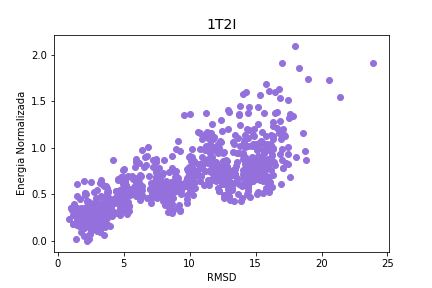
\includegraphics[width=0.7\textwidth]{images/1t2i_tunnel.png}
    \end{figure}
    
    \begin{equation*}
        E_{i(norm)} = \frac{E_i - E_{\min}}{E_{95th} - E_{5th}},
    \end{equation*}
\end{frame}

\begin{frame}{Ranking de Energia}
    \begin{table}[]
    \centering
    \caption{Rank mostrando as top 5 decoys dos experimentos com a proteína 1T2I.}
    \label{tab:protrank}
    \begin{tabular}{@{}ccc@{}}
        \toprule
        Rank & Energia Normalizada & RMSD  \\
        \midrule
        1    & 0.000             & 2.233 \\
        2    & 0.023             & 1.37  \\
        3    & 0.025             & 2.395 \\
        4    & 0.057             & 2.004 \\
        5    & 0.061             & 2.356 \\
        \bottomrule
    \end{tabular}
\end{table}
\end{frame}

\begin{frame}{VAE e ciclos ótimos}
    \begin{figure}
        \centering
        \begin{minipage}{0.45\textwidth}
            \centering
            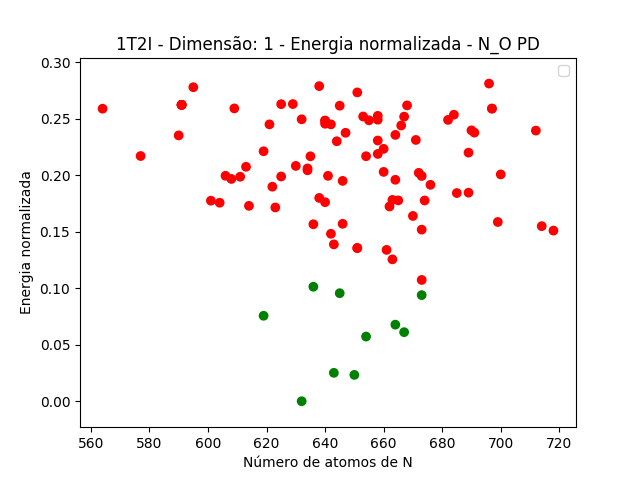
\includegraphics[width=1.1\textwidth]{images/cyc1t2iN.png} % first figure itself
        \end{minipage}\hfill
        \begin{minipage}{0.45\textwidth}
            \centering
            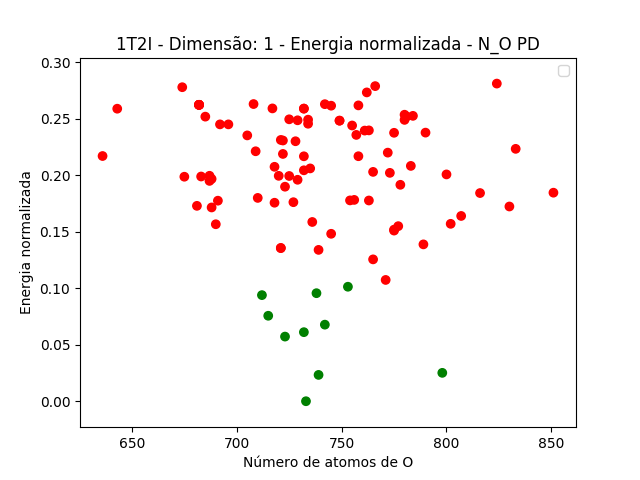
\includegraphics[width=1.1\textwidth]{images/cyc1t2iO.png} % second figure itself
        \end{minipage}
        \caption{Soma dos átomos de nitrogênio (esquerda) e oxigênio (direita) que compõe os ciclos do 
        $1^\circ$ diagrama de persistência das decoys da proteína 1T2I.}
    \end{figure}
    %\begin{figure}
    %\centering
    %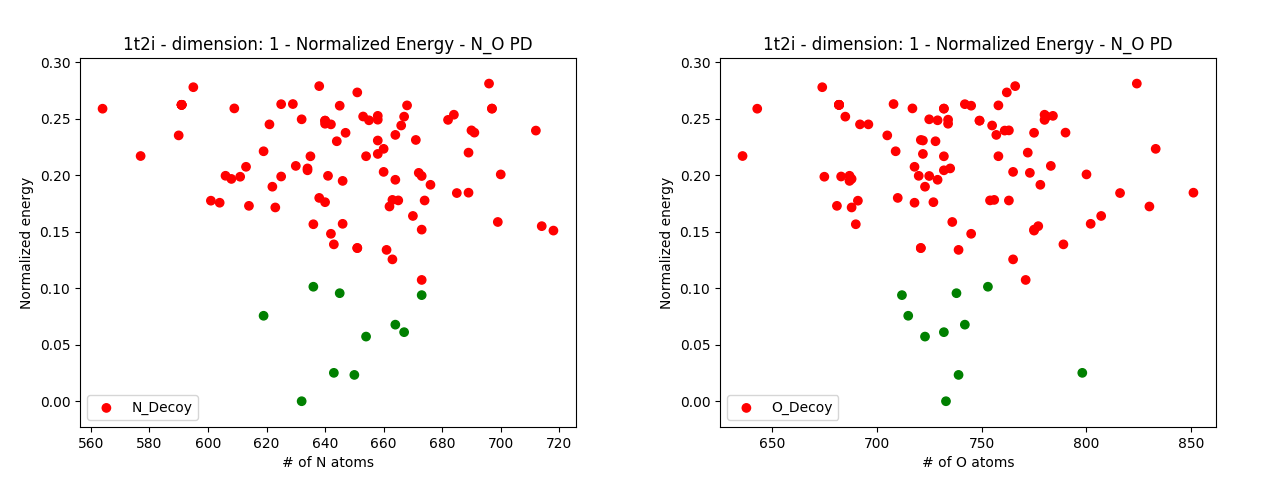
\includegraphics[width=0.8\textwidth]{../images/relatorio/NOcyc.png}
    %\caption{Soma dos átomos de nitrogênio (esquerda) e oxigênio (direita) que compõe os ciclos do 
    %$1^\circ$ diagrama de persistência das decoys da proteína 1T2I.}
    %\end{figure}
\end{frame}

\begin{frame}{VAE e ciclos ótimos}
    \begin{figure}
    \centering
    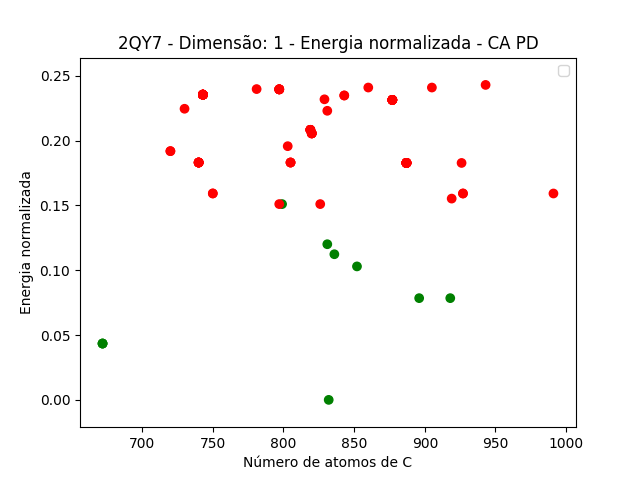
\includegraphics[width=0.8\textwidth]{images/cyc2qy7.png}
    \caption{Soma dos átomos de carbono que compõem os ciclos do
            $1^\circ$ diagrama de persistência das decoys da 2QY7.}
    \end{figure}
\end{frame}

\begin{frame}{Prevendo o RMSD}
    \begin{figure}
    \centering
    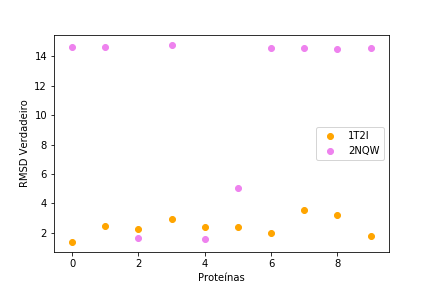
\includegraphics[width=0.8\textwidth]{images/true_rmsd.png}
    \caption{Valor do RMSD para cada decoy no top 10. Não existem falsos mínimos para a proteína 1T2I, enquanto
    isso existem 7 falsos mínimos para a proteína 2NQW.}
    \label{fig:truermsd}
\end{figure}
\end{frame}

\begin{frame}{Resultados}
    \begin{table}[!htbp]
     \centering
     \caption{Melhores parâmetros para cada métrica para os regressores treinados nas imagens de persistência.}
     \label{tab:bestruns}
     \begin{tabular}{@{}cccccc@{}}
     \toprule
     \textbf{Métrica} & \textbf{Regressor} & \textbf{Pixel} & \textbf{Var.} &
     \textbf{Átomos}\footnote{Átomos utilizados para calcular os diagramas de persistência. "todo" significa
     que todos os átomos menos os de hidrogênio foram usados para os PD's.}
      & Score médio
     \\
     \midrule
     $R^2$           & Redes neurais     & 100       & 1,0             & C     & $-5,780$ \\
     MSE             & Redes neurais     & 100       & 1,0             & C     &  $8,299$  \\
     RMSE            & Reg. lin c/ reg.   & 10    & 1,2           & todo  &  $2,599$  \\
         Acur. Bin. & GBoost             & 10      & 0,6             & N,O   &  $0,657$  \\
     \bottomrule
     \end{tabular}
\end{table}
\end{frame}

\begin{frame}{Resultados}
\begin{table}[!htbp]
    \centering
    \caption{Melhores regressores treinados com as propriedades das proteínas}.
    \label{tab:rosregr}
    \begin{tabular}{@{}ccc@{}}
        \toprule
        \textbf{Métrica} & \textbf{Regressor} & \textbf{Score médio} \\ \midrule
        $R^2$           & Random Forest II       &-13,706        \\
        MSE             & Random Forest II       & 10,113         \\
        RMSE            & Random Forest II        & 2,707          \\
        Acurácia binária & Regressão lin. c/ reg. & 0,586          \\ \bottomrule
    \end{tabular}
\end{table}
\end{frame}

\begin{frame}{Resultados}
\begin{figure}
    \centering
    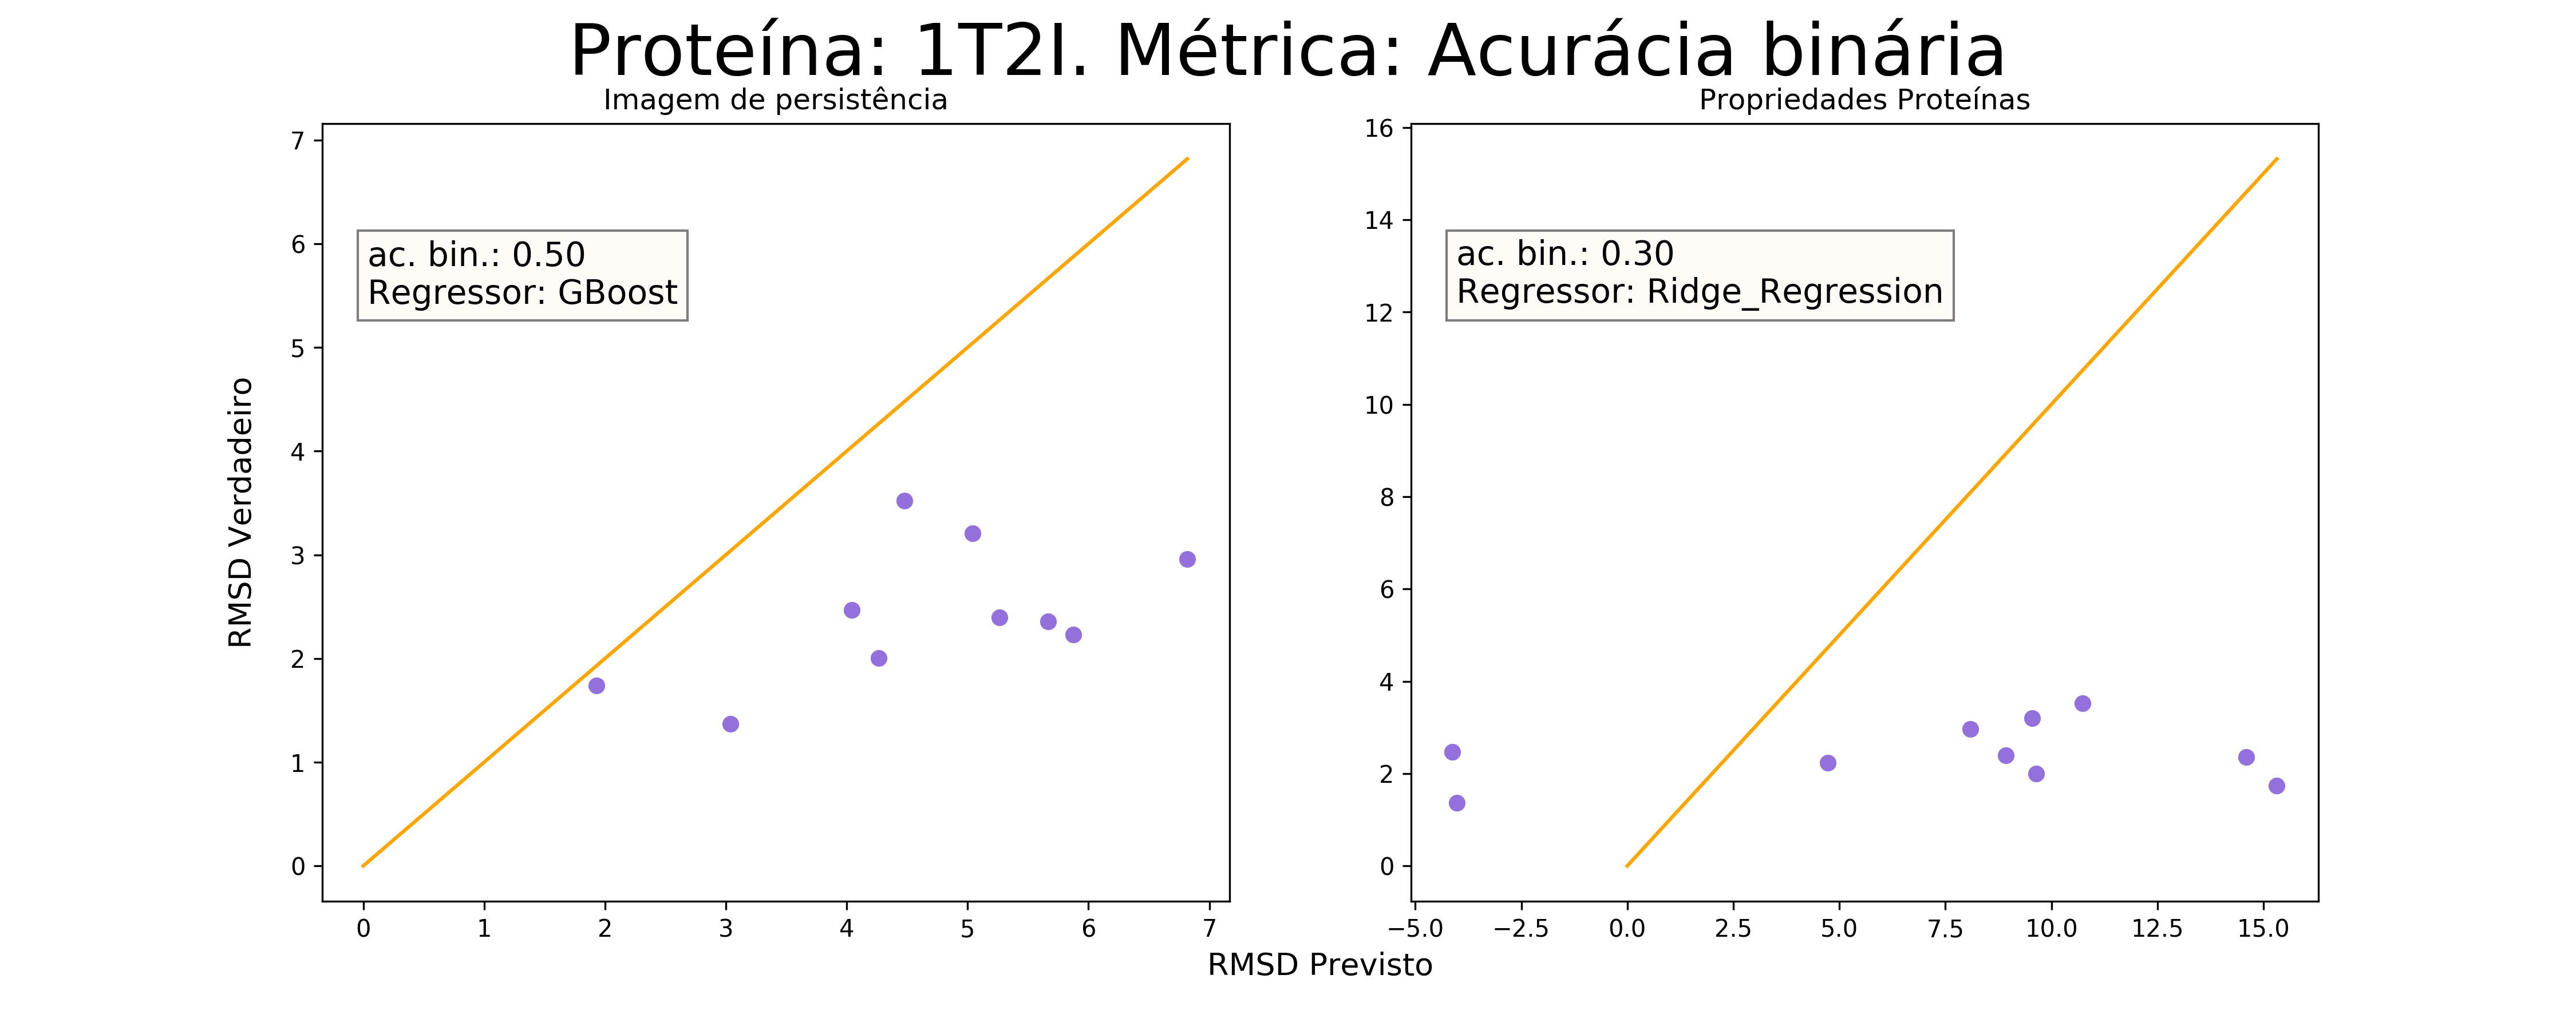
\includegraphics[width=1.0\textwidth]{images/1t2i_binary.png}
    \caption{RMSD previsto x RMSD verdadeiro para o top 10 decoys da proteína 1T2I dados os
             regressores com a melhor acurácia binária no conjunto de validação. Na 
            esquerda os valores para regressores treinados com PI's, já na esquerda com propriedades
            das proteínas.}
    \label{fig:1t2i_binary}
\end{figure}
\end{frame}

\section{Conclusão}

\begin{frame}{Conclusão}
    \begin{itemize}
        \item Análise topológica de dados é uma área flexível e que pode ser aplicada em proteínas;
        \item Muitas propriedades biológicas das proteínas podem ser detectadas pelos respectivos ciclos
         do diagrama de persistência.
    \end{itemize}
\end{frame}

\begin{frame}{Agradecimentos}
    \begin{itemize}
        \pause
        \item Marcio Gameiro
        \pause
        \item Konstantin Mischaikow
        \item Lun Zhang
        \pause
        \item Priscila Cavassin
        \pause
        \item E a todos os amigos.
    \end{itemize} 
\end{frame}

\section{Referências}

\begin{frame}[allowframebreaks]{Referências}
  
    \nocite{*}
    \bibliography{ref}
 
\end{frame}

\end{document}
